\documentclass[a4paper,12pt]{scrartcl}
\usepackage{url}                      %% weblinks
\usepackage{longtable}                %% make tables look nice
\usepackage{multirow}                 %% for \multirow and \multicolumn commands
\usepackage{hyperref}                 %% in document links
\usepackage{graphicx}                 %% figures


%% Bibliography-----------------------------------
\usepackage[sorting=none, backend=bibtex8]{biblatex}
\usepackage{csquotes}
\addbibresource{refs.bib}


\begin{document}

\section{Quick Explanation about SLAM's front and back-ends}
SLAM algorithms are mostly separated into a front-end and a back-end \cite{Cadena2016}. Using this separation
the front-end resembles the part of the program which interprets the sensor data by e.g. extracting landmarks and executing
data association\footnote{Matching landmark between frames.}. The back-end on the other hand describes the part of the
algorithm which is responsible for estimating the robot's pose and the map (i.e. the landmark locations). Figure
\ref{fig:slam_front_and_back_end} sketches this relationship for a typical SLAM system.

\begin{figure}[htbp]
    \begin{center}
        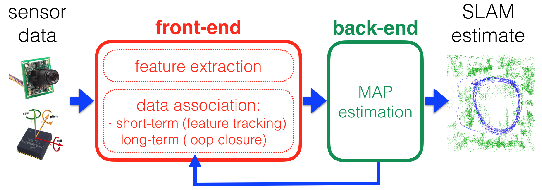
\includegraphics[width=\textwidth]{slam_front_and_back_end.pdf}
    \end{center}
    \caption{Front-end and back-end in a typical SLAM system. The back-end can provide feedback to the front-end for loop
    closure detection. \cite{Cadena2016}}
    \label{fig:slam_front_and_back_end}
\end{figure}


\newpage
\begin{longtable}{c| l l}
  \caption{Monocular graph-based SLAM approaches}\\
  \label{tab:slam_overview}
    \textbf{Name}        & \multicolumn{2}{l}{\textbf{Characteristics}}                                                                              \\
    \hline                                                                                                                                           \\ [-3mm]
    \multirow{8}{5em}{\textbf{CD-SLAM}} & \textit{Front-end:}    & Histogram of Oriented Cameras (HoC) descriptor \cite{Pirker2010}                  \\
                                        & \textit{Back-end:}     & Keyframe-based BA, graph optimization                                             \\
                                        & \textit{Loop closing:} & Yes, using FAB-MAP                                                                \\
                                        & \textit{Code:}         & -                                                                                 \\
                                        & \textit{Refs(year):}   & \cite{Pirker2011}(2011)                                                           \\
                                        & \textit{Notes:}        & \multirow{3}{24em}{Focus on highly dynamic environments,                          \\
                                                                               Keep map proportional to explored space not time,                     \\
                                                                               Usage of HoC descriptor in feature based front end}                   \\
                                        &                                                                                                            \\
                                        &                                                                                                            \\ [2mm]
    \hline                                                                                                                                           \\ [-3mm]
    \multirow{7}{5em}{\textbf{C-KLAM}} & \textit{Front-end:}    & SIFT features                                                                      \\
                                       & \textit{Back-end:}     & Custom to C-KLAM, based on BA                                                      \\
                                       & \textit{Loop closing:} & Possible, but was not achieved in test                                             \\
                                       & \textit{Code:}         & -                                                                                  \\
                                       & \textit{Refs(year):}   & \cite{Nerurkar2014}(2014)                                                          \\
                                       & \textit{Notes:}        & \multirow{2}{24em}{Focus on making use of  data between keyframes,                 \\
                                                                               Incorporates IMU data in graph optimization}                          \\
                                       &                                                                                                             \\ [2mm]
    \hline                                                                                                                                           \\ [-3mm]
    \multirow{10}{5em}{\textbf{CNN SLAM}} & \textit{Front-end:}    & Dense approach based on LSD SLAM                                                \\
                                          & \textit{Back-end:}     & $Sim(3)$ optimization and BA                                                    \\
                                          & \textit{Loop closing:} & Not mentioned in paper                                                          \\
                                          & \textit{Code:}         & -                                                                               \\
                                          & \textit{Refs(year):}   & \cite{Tateno2017}(2017)                                                         \\
                                          & \textit{Notes:}        & \multirow{5}{24em}{Uses trained CNN to predict depth maps,                      \\
                                                                                 Can be used to correct scale drift,                                 \\
                                                                                 Relies on use of GPU,                                               \\
                                                                                 Implements semantic labeling (i.e. distinguish walls and floor)}    \\
                                          &                                                                                                          \\
                                          &                                                                                                          \\
                                          &                                                                                                          \\
                                          &                                                                                                          \\ [2mm]
    \hline                                                                                                                                           \\ [-3mm]
    \multirow{9}{5em}{\textbf{COP SLAM}} & \textit{Front-end:}    & Any front-end that creates pose-graphs                                           \\
                                         & \textit{Back-end:}     & Optimizing pose-chains using trajectory bending\cite{Dubbelman2010}              \\
                                         & \textit{Loop closing:} & Is a back-end $\rightarrow$ no detection, only optimization                      \\
                                         & \textit{Code:}         & -                                                                                \\
                                         & \textit{Refs(year):}   & \cite{Dubbelman2013}(2013), \cite{Dubbelman2015}(2015)                           \\
                                         & \textit{Notes:}        & \multirow{4}{24em}{Optimizes sparse pose-graph (pose-chain),                     \\
                                                                                 50 to 200 times faster than G$^2$O,                                 \\
                                                                                 Only optimizes the robot pose, not the map,                         \\
                                                                                 Has an extension which can account for scale-drift}                 \\
                                         &                                                                                                           \\
                                         &                                                                                                           \\
                                         &                                                                                                           \\
    \newpage
    \multirow{8}{5em}{\textbf{Dolphin-SLAM}} & \textit{Front-end:}    & Sensor dependant, Sonar: HU moments, Image: SURF                             \\
                                             & \textit{Back-end:}     & RatSLAM back-end (not really graph-based)                                    \\
                                             & \textit{Loop closing:} & Yes, using FAB-MAP                                                           \\
                                             & \textit{Code:}         & \url{https://github.com/dolphin-slam/dolphin\_slam}                          \\
                                             & \textit{Refs(year):}   & \cite{Silveira2015}(2015), \cite{Zaffari2016}(2016)                          \\
                                             & \textit{Notes:}        & \multirow{3}{24em}{Focus on SLAM in underwater scenario,                     \\
                                                                                 Multiple sensors: sonar, camera, IMU and DVL,                       \\
                                                                                 Based on RatSLAM}                                                   \\
                                             &                                                                                                       \\
                                             &                                                                                                       \\ [2mm]
    \hline                                                                                                                                           \\ [-3mm]
    \multirow{9}{5em}{\textbf{DPPTAM}} & \textit{Front-end:}    & Piecewise planar dense                                                             \\
                                       & \textit{Back-end:}     & \multirow{2}{24em}{Semi-dense map with estimation of
                                                                         planar surfaces, map optimization not mentioned}                            \\
                                       &                                                                                                             \\
                                       & \textit{Loop closing:} & Not mentioned in paper                                                             \\
                                       & \textit{Code:}         & \url{https://github.com/alejocb/dpptam}                                            \\
                                       & \textit{Refs(year):}   & \cite{Concha2015b}(2015)                                                           \\
                                       & \textit{Notes:}        & \multirow{4}{24em}{Reconstruction of dense maps using only CPU,                    \\
                                                                         Reduced cost due to planar surface estimation via superpixels \cite{Felzenszwalb2015}
                                                                         with the assumption that low color-gradient areas are mostly planar}        \\
                                       &                                                                                                             \\
                                       &                                                                                                             \\
                                       &                                                                                                             \\ [2mm]
    \hline                                                                                                                                           \\ [-3mm]
    \multirow{9}{5em}{\textbf{DSO}} & \textit{Front-end:}    & Sparse and direct                                                                     \\
                                    & \textit{Back-end:}     & None (odometry only)                                                                  \\
                                    & \textit{Loop closing:} & No                                                                                    \\
                                    & \textit{Code:}         & \url{https://github.com/JakobEngel/dso}                                               \\
                                    & \textit{Refs(year):}   & \cite{Concha2015b}(2015)                                                              \\
                                    & \textit{Notes:}        & \multirow{4}{24em}{Optimizes camera intrinsics and extrinsics,                        \\
                                                                      Works well in low textured areas,                                              \\
                                                                      Distributes sampled pixels such that, when available, high gradients
                                                                      are used, otherwise takes weak gradients}                                      \\
                                    &                                                                                                                \\
                                    &                                                                                                                \\
                                    &                                                                                                                \\ [2mm]
    \hline                                                                                                                                           \\ [-3mm]
    \multirow{8}{5em}{\textbf{DTAM}} & \textit{Front-end:}    & Dense method                                                                         \\
                                     & \textit{Back-end:}     & Creates dense map, no graph optimization                                             \\
                                     & \textit{Loop closing:} & No                                                                                   \\
                                     & \textit{Code:}         & \url{https://github.com/anuranbaka/OpenDTAM}                                         \\
                                     & \textit{Refs(year):}   & \cite{Newcombe2011}(2011)                                                            \\
                                     & \textit{Notes:}        & \multirow{3}{24em}{Relies on GPU for computation,                                    \\
                                                                      Creates feature-rich, textured, dense map,                                     \\
                                                                      Robust against quick movement and camera defocus}                              \\
                                     &                                                                                                               \\
                                     &                                                                                                               \\ [2mm]
    \newpage
    \multirow{10}{5em}{\textbf{DT SLAM}} & \textit{Front-end:}    & FAST, separated 2D and 3D feature matching                                       \\
                                         & \textit{Back-end:}     & BA on pose and features of all sub maps                                          \\
                                         & \textit{Loop closing:} & Yes                                                                              \\
                                         & \textit{Code:}         & \url{https://github.com/plumonito/dtslam}                                        \\
                                         & \textit{Refs(year):}   & \cite{Daniel2014}(2014)                                                          \\
                                         & \textit{Notes:}        & \multirow{5}{24em}{Holds off 3D feature triangulation
                                                                                until enough parallax is observed
                                                                                (Deferred triangulation),                                            \\
                                                                                Can incorporate purely rotational movement frames,                   \\
                                                                                Creates sub-maps which can be merged later to avoid
                                                                                scale inconsistencies}                                               \\
                                         &                                                                                                           \\
                                         &                                                                                                           \\
                                         &                                                                                                           \\
                                         &                                                                                                           \\
    \hline                                                                                                                                           \\ [-3mm]
    \multirow{10}{5em}{\textbf{FAB-MAP}} & \textit{Front-end:}    & Appearance-based bag of words approach with SURF                                 \\
                                         & \textit{Back-end:}     & Place recognition in appearance-space, no metric map                             \\
                                         & \textit{Loop closing:} & Yes                                                                              \\
                                         & \textit{Code:}         & \url{https://github.com/arrenglover/openfabmap}                                  \\
                                         & \textit{Refs(year):}   & \cite{Cummins2008}(2008), \cite{Cummins2009}(2009),
                                                                            \cite{Glover2012}(2012)                                                  \\
                                         & \textit{Notes:}        & \multirow{5}{24em}{Needs training on an environment similar to
                                                                            the one it is going to be used in,                                       \\
                                                                            Place recognition via visual bag of words database,                      \\
                                                                            No metric map creation, mostly used as a tool for
                                                                            loop closure detection in other approaches like LSD SLAM}                \\
                                         &                                                                                                           \\
                                         &                                                                                                           \\
                                         &                                                                                                           \\
                                         &                                                                                                           \\ [2mm]
    \hline                                                                                                                                           \\ [-3mm]
    \multirow{8}{5em}{\textbf{LSD SLAM}} & \textit{Front-end:}    & Semi-dense                                                                       \\
                                         & \textit{Back-end:}     & Creates semi-dense map, pose-graph optimization (g2o)                            \\
                                         & \textit{Loop closing:} & Yes, small via $sim(3)$ and large via FAB-MAP                                    \\
                                         & \textit{Code:}         & \url{https://github.com/tum-vision/lsd_slam}                                     \\
                                         & \textit{Refs(year):}   & \cite{Engel2013}(2013), \cite{Engel2014}(2014)                                   \\
                                         & \textit{Notes:}        & \multirow{3}{24em}{Semi-dense, keyframe-based, runs on CPU,                      \\
                                                                                 Makes use of Lie-algebra for tracking and optimization,             \\
                                                                                 Scale-drift aware}                                                  \\
                                         &                                                                                                           \\
                                         &                                                                                                           \\ [2mm]
    \hline                                                                                                                                           \\ [-3mm]
    \multirow{8}{5em}{\textbf{NID SLAM}} & \textit{Front-end:}    & Semi-dense, NID metric                                                           \\
                                         & \textit{Back-end:}     & Creates semi-dense map, pose-graph optimization (g2o)                            \\
                                         & \textit{Loop closing:} & Yes, using FAB-MAP                                                               \\
                                         & \textit{Code:}         & -                                                                                \\
                                         & \textit{Refs(year):}   & \cite{Pascoe2017}(2017)                                                          \\
                                         & \textit{Notes:}        & \multirow{3}{24em}{Focus on lighting, weather and structural changes,            \\
                                                                                 Relies on GPU for computation,                                      \\
                                                                                 Scale-drift aware (based on LSD SLAM)}                              \\
                                         &                                                                                                           \\
                                         &                                                                                                           \\ [2mm]
    \newpage
    \multirow{10}{5em}{\textbf{ORB SLAM}} & \textit{Front-end:}    & Indirect using ORB feature descriptor                                           \\
                                          & \textit{Back-end:}     & BA on sub-graphs, uses local maps                                               \\
                                          & \textit{Loop closing:} & Yes, using a place recognition database                                         \\
                                          & \textit{Code:}         & \url{https://github.com/raulmur/ORB_SLAM}                                       \\
                                          & \textit{Refs(year):}   & \cite{Mur-Artal2015}(2015)                                                      \\
                                          & \textit{Notes:}        & \multirow{5}{24em}{Uses three parallel threads for
                                                                                 tracking, local map creation and loop closing,                      \\
                                                                                 Uses a bag of words approach for place recognition,                 \\
                                                                                 Focus on real-time operation, runs on CPU,                          \\
                                                                                 Focus on long-term localization, not detailed maps}                 \\
                                          &                                                                                                          \\
                                          &                                                                                                          \\
                                          &                                                                                                          \\
                                          &                                                                                                          \\ [2mm]
    \hline                                                                                                                                           \\ [-3mm]
    \multirow{7}{5em}{\textbf{ORB SLAM2}} & \textit{Front-end:}    & Indirect using ORB feature descriptor                                           \\
                                          & \textit{Back-end:}     & BA on sub-graphs, uses local maps                                               \\
                                          & \textit{Loop closing:} & Yes, using a place recognition database                                         \\
                                          & \textit{Code:}         & \url{https://github.com/raulmur/ORB_SLAM2}                                      \\
                                          & \textit{Refs(year):}   & \cite{Mur-Artal2016a}(2016)                                                     \\
                                          & \textit{Notes:}        & \multirow{2}{24em}{Extension of ORB SLAM
                                                                                 for RGB-D and stereo camera setups}                                 \\
                                          &                                                                                                          \\ [2mm]
    \hline                                                                                                                                           \\ [-3mm]
    \multirow{8}{5em}{\textbf{Visual Inertial ORB SLAM}} & \textit{Front-end:}    & Indirect using ORB feature descriptor                            \\
                                                         & \textit{Back-end:}     & BA on sub-graphs, uses local maps                                \\
                                                         & \textit{Loop closing:} & Yes, using a place recognition database                          \\
                                                         & \textit{Code:}         & -                                                                \\
                                                         & \textit{Refs(year):}   & \cite{Mur-Artal2017}(2017)                                       \\
                                                         & \textit{Notes:}        & \multirow{4}{24em}{Modular extension of ORB SLAM
                                                                                                for incorporating IMU readings,                      \\
                                                                                                Takes gyroscope and accelerometer bias into account, \\
                                                                                                Derives scale from IMU measurements}                 \\
                                                         &                                                                                           \\
                                                         &                                                                                           \\
                                                         &                                                                                           \\ [2mm]
    \hline                                                                                                                                           \\ [-3mm]
    \multirow{9}{5em}{\textbf{PTAM}} & \textit{Front-end:}    & Indirect, using FAST corner detector                                                 \\
                                     & \textit{Back-end:}     & Local and global BA                                                                  \\
                                     & \textit{Loop closing:} & No                                                                                   \\
                                     & \textit{Code:}         & \url{https://github.com/Oxford-PTAM/PTAM-GPL}                                        \\
                                     & \textit{Refs(year):}   & \cite{Klein2007}(2007)                                                               \\
                                     & \textit{Notes:}        & \multirow{4}{24em}{First to parallelize tracking and mapping,                        \\
                                                                      Uses keyframes to create map,                                                  \\
                                                                      Optimizes map in background when exploring
                                                                      already known areas}                                                           \\
                                     &                                                                                                               \\
                                     &                                                                                                               \\
                                     &                                                                                                               \\ [2mm]
    \newpage
    \multirow{9}{5em}{\textbf{Rat-SLAM}} & \textit{Front-end:}    & Not specified                                                                    \\
                                         & \textit{Back-end:}     & Neural network based on the hippocampus of rodents                               \\
                                         & \textit{Loop closing:} & Yes, via local view cells                                                        \\
                                         & \textit{Code:}         & \url{https://github.com/davidmball/ratslam}                                      \\
                                         & \textit{Refs(year):}   & \cite{Milford2004}(2004), \cite{Milford2005}(2005), \cite{Milford2006}(2006),
                                                                    \cite{Milford2008}(2008),  \cite{Ball2013}(2013)                                 \\
                                         & \textit{Notes:}        & \multirow{4}{24em}{Back-end that can make use of different input data
                                                                          both visual and internal (IMU),                                            \\
                                                                          Composed of pose cells, local view cells, and
                                                                          experience map}                                                            \\
                                         &                                                                                                           \\
                                         &                                                                                                           \\
                                         &                                                                                                           \\
    \hline                                                                                                                                           \\ [-3mm]
    \multirow{10}{5em}{\textbf{RD SLAM}} & \textit{Front-end:}    & Indirect, using SIFT                                                             \\
                                         & \textit{Back-end:}     & BA based on PTAM                                                                 \\
                                         & \textit{Loop closing:} & No                                                                               \\
                                         & \textit{Code:}         & \url{http://www.zjucvg.net/rdslam/rdslam.html}                                   \\
                                         & \textit{Refs(year):}   & \cite{Tan2013a}(2013)                                                            \\
                                         & \textit{Notes:}        & \multirow{5}{24em}{Based on PTAM,                                                \\
                                                                                Focus on dynamic environments with changes in structure
                                                                                and illumination,                                                    \\
                                                                                According to author still fails frequently,                          \\
                                                                                Relies on GPU due to SIFT features}                                  \\
                                         &                                                                                                           \\
                                         &                                                                                                           \\
                                         &                                                                                                           \\
                                         &                                                                                                           \\ [2mm]
    \hline                                                                                                                                           \\ [-3mm]
    \multirow{9}{5em}{\textbf{REBVO}} & \textit{Front-end:}    & Between direct and indirect, using edges as features                                \\
                                      & \textit{Back-end:}     & None (odometry only)                                                                \\
                                      & \textit{Loop closing:} & No                                                                                  \\
                                      & \textit{Code:}         & \url{https://github.com/JuanTarrio/rebvo}                                           \\
                                      & \textit{Refs(year):}   & \cite{Tarrio2016}(2016)                                                             \\
                                      & \textit{Notes:}        & \multirow{4}{24em}{Tracks edges instead of features or pixels,                      \\
                                                                          Focus on running on embedded devices,                                      \\
                                                                          Has extension for IMU integration,                                         \\
                                                                          Depth estimated via EKF}                                                   \\
                                      &                                                                                                              \\
                                      &                                                                                                              \\
                                      &                                                                                                              \\ [2mm]
    \hline                                                                                                                                           \\ [-3mm]
    \multirow{8}{5em}{\textbf{REMODE}} & \textit{Front-end:}    & Direct, dense method, bayesian estimation for depth                                \\
                                       & \textit{Back-end:}     & Creates dense map, no graph optimization                                           \\
                                       & \textit{Loop closing:} & No                                                                                 \\
                                       & \textit{Code:}         & \url{https://github.com/uzh-rpg/rpg_open_remode}                                   \\
                                       & \textit{Refs(year):}   & \cite{Pizzoli2014}(2014)                                                           \\
                                       & \textit{Notes:}        & \multirow{3}{24em}{Depth estimation via a bayesian scheme,                         \\
                                                                          Can smooth camera measurement noise,                                       \\
                                                                          Relies on GPU for processing}                                              \\
                                       &                                                                                                             \\
                                       &                                                                                                             \\ [2mm]
    \newpage
    \multirow{8}{5em}{\textbf{RFM SLAM}} & \textit{Front-end:}    & Indirect, but not specified which features                                       \\
                                         & \textit{Back-end:}     & Splits orientation and position estimation for 2D case                           \\
                                         & \textit{Loop closing:} & Yes                                                                              \\
                                         & \textit{Code:}         & -                                                                                \\
                                         & \textit{Refs(year):}   & \cite{Agarwal2016}(2016)                                                         \\
                                         & \textit{Notes:}        & \multirow{3}{24em}{Separates orientation and position estimation,                \\
                                                                                  2D case can be extended to 3D,                                     \\
                                                                                  Focus on computationally cheaper pose optimization}                \\
                                         &                                                                                                           \\
                                         &                                                                                                           \\ [2mm]
    \hline                                                                                                                                           \\ [-3mm]
    \multirow{8}{5em}{\textbf{RK SLAM}}  & \textit{Front-end:}    & Indirect, FAST, uses homographies for tracking                                   \\
                                         & \textit{Back-end:}     & Local and global optimization using BA                                           \\
                                         & \textit{Loop closing:} & Yes                                                                              \\
                                         & \textit{Code:}         & \url{http://www.zjucvg.net/rkslam/rkslam.html}                                   \\
                                         & \textit{Refs(year):}   & \cite{Liu2016}(2016)                                                             \\
                                         & \textit{Notes:}        & \multirow{3}{24em}{Focus on fast motion and rotation,                            \\
                                                                                  Extracts and matches 3D planes in keyframes,                       \\
                                                                                  Has extension to incorporate IMU data}                             \\
                                         &                                                                                                           \\
                                         &                                                                                                           \\
                                         &                                                                                                           \\ [-5mm]
    \hline                                                                                                                                           \\ [-3mm]
    \multirow{8}{5em}{\textbf{Seq SLAM}} & \textit{Front-end:}    & Looks for minimum in difference of image sequences                               \\
                                         & \textit{Back-end:}     & No map creation or localization, only place recognition                          \\
                                         & \textit{Loop closing:} & Yes                                                                              \\
                                         & \textit{Code:}         & \url{https://github.com/subokita/OpenSeqSLAM}                                    \\
                                         & \textit{Refs(year):}   & \cite{Milford2012}(2012)                                                         \\
                                         & \textit{Notes:}        & \multirow{3}{24em}{Focus on extreme changes in environment,                      \\
                                                                             Like FAB-MAP no real SLAM approach which localizes
                                                                             a robot and builds a map, rather used for loop closure}                 \\
                                         &                                                                                                           \\
                                         &                                                                                                           \\
                                         &                                                                                                           \\
    \hline                                                                                                                                           \\ [-3mm]
    \multirow{8}{5em}{\textbf{SVO}}    & \textit{Front-end:}    & Semi-direct, dense pixel batches and FAST                                          \\
                                       & \textit{Back-end:}     & BA for pose, keeps a small map of fixed size                                       \\
                                       & \textit{Loop closing:} & No                                                                                 \\
                                       & \textit{Code:}         & \url{https://github.com/uzh-rpg/rpg_svo}                                           \\
                                       & \textit{Refs(year):}   & \cite{Forster2014a}(2014), \cite{Forster2017}(2017)                                \\
                                       & \textit{Notes:}        & \multirow{3}{24em}{Focus on runtime, runs on embedded devices,                     \\
                                                                             Comes with two settings: \textit{fast} and \textit{accurate},           \\
                                                                            Fixed number of keyframes in map,                                        \\
                                                                            Needs high FPS $\sim$ 60 FPS}                                            \\
                                       &                                                                                                             \\
                                       &                                                                                                             \\
                                       &                                                                                                             \\ [-5mm]
\end{longtable}


\newpage
%Bibiliography
\printbibliography

\end{document}
